\subsection{One hot encoding i korelacje}
Jak wspomniano we wstępie, dla zadań klayfikacji binarnej wykonany został \textbf{One Hot Encoding} kolumny \textbf{Type\_Of\_Renewable\_Energy}. Ze względu na problemy ze środowiskiem wykonawczym, odpowiednia funkcja została napisana bez użycia zewnętrznych bibliotek:

\begin{Rcode}
unique_types <- unique(energy_data$Type_of_Renewable_Energy)

for (type in unique_types) {
  column_name <- paste("Type_of_Renewable_Energy", type, sep = "_")
  energy_data[[column_name]] <- ifelse(energy_data$Type_of_Renewable_Energy == type, 1, 0)
}

energy_data <- subset(energy_data, select = -c(Type_of_Renewable_Energy))
\end{Rcode}

Otrzymujemy w ten sposób 7 dodatkowych kolumn o binarnych wartościach, które zostaną użyte jako cel klasyfikacji.

Znajdźmy najsilniejsze korelacje między cechami (pomijając korelacje między tymi samymi cechami):

\begin{Rcode}
numeric_data <- energy_data[sapply(energy_data, is.numeric)]
corr_mat <- cor(numeric_data)
corr_df <- as.data.frame(as.table(corr_mat))
corr_df <- corr_df[corr_df$Var1 != corr_df$Var2,]
corr_df <- corr_df[order(abs(corr_df$Freq)),]
top_corrs <- head(corr_df, 10)
\end{Rcode}

\begin{figure}[H]
    \centering
    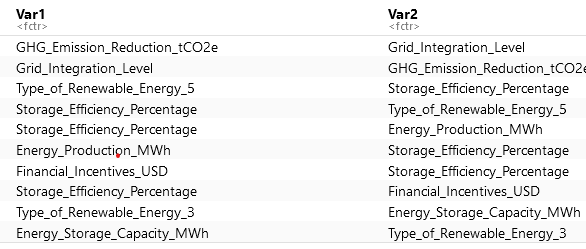
\includegraphics[width=1\linewidth]{lab2/obraz.png}
    \caption{Zmienne o najwyższych korelacjach.}
    \label{fig:enter-label}
\end{figure}

\subsection{Regresja logistyczna}

Spróbujmy przywidzieć czy dane źródło energii należy do \textbf{1 kategorii} za pomocą zmiennych \textbf{Installed\_Capacity\_MW}, \textbf{Energy\_Production\_MWh}, \textbf{Energy\_Storage\_Capacity\_MWh} i \textbf{Storage\_Efficiency\_Percentage}.

\begin{Rcode}
dir_logistic <- list()
dir_logistic$fit <- glm(Type_of_Renewable_Energy_1 ~ Installed_Capacity_MW + Energy_Production_MWh 
                        + Energy_Storage_Capacity_MWh + Storage_Efficiency_Percentage, 
                   family = binomial, data = energy_data)
dir_logistic$predicted <- ifelse(dir_logistic$probs > 0.5, "Type 1", "Not type 1")
dir_logistic$cm <- table(dir_logistic$predicted, energy_data$Type_of_Renewable_Energy_1)
dir_logistic$cm
\end{Rcode}

Otrzymujemy wyniki:
\begin{figure}[H]
    \centering
    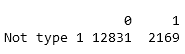
\includegraphics[width=0.7\linewidth]{lab2/obraz3.png}
    \caption{Nienależność i należność do badanej klasy}
    \label{fig:enter-label}
\end{figure}

Finalnie otrzymaliśmy proporcję błędów treningowych równą 0 - być może zadanie jest zbyt trywialne. Sprawdźmy jak wyniki zmieni poprawny podział zbioru.

\subsection{Podział zbioru}
Losowo dzielimy zbiór na treningowy i testowy w proporcjach 70/30:

\begin{Rcode}
set.seed(123)

train_indices <- sample(nrow(energy_data), round(0.7 * nrow(energy_data)))
train <- energy_data[train_indices, ]
energy_data_test <- energy_data[-train_indices, ]
Type_of_Renewable_Energy_1_test <- energy_data_test$Type_of_Renewable_Energy_1
\end{Rcode}

Wykonujemy regresję na zbiorze treningowym:

\begin{Rcode}
dir_log_t <- list()
dir_log_t$fit <- glm(Type_of_Renewable_Energy_1 ~ Installed_Capacity_MW + Energy_Production_MWh, 
                   family = binomial, data = train)
\end{Rcode}

\begin{figure}[H]
    \centering
    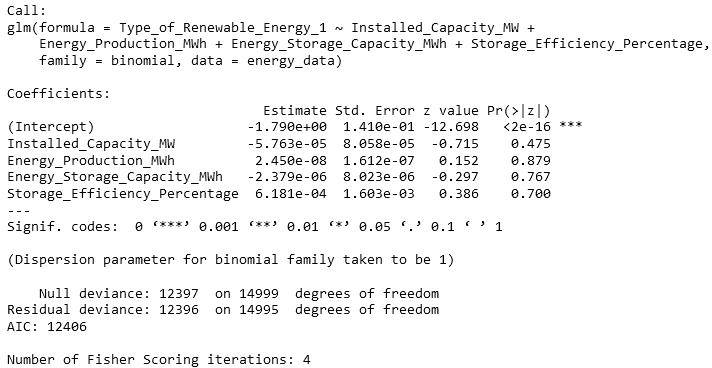
\includegraphics[width=1\linewidth]{lab2/obraz4.png}
    \caption{Podsumowanie regresji na zbiorze treningowym.}
    \label{fig:enter-label}
\end{figure}

Sprawdźmy predykcje na zbiorze testowym:

\begin{Rcode}
dir_log_t$probs <- predict(dir_log_t$fit, energy_data_test, type = "response")
dir_log_t$predicted <- ifelse(dir_log_t$probs > 0.5, "Type 1", "Not type 1")
table(dir_log_t$predicted, Type_of_Renewable_Energy_1_test)
\end{Rcode}

\begin{figure}[H]
    \centering
    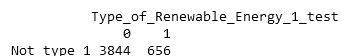
\includegraphics[width=0.75\linewidth]{lab2/obraz5.png}
    \caption{Macierz pomyłek}
    \label{fig:enter-label}
\end{figure}

W tym przypadku otrzymaliśmy proprocję błędów na poziomie około 20\%.

Użyjmy predyktorów mocniej skorelowanych ze zmienną objaśnianą, czyli \textbf{Energy\_Production\_MWh} i \textbf{Energy\_Storage\_Capacity\_MWh}:

\begin{Rcode}
dir_log_best2$fit <- glm(Type_of_Renewable_Energy_1 ~ Installed_Capacity_MW + Energy_Production_MWh, 
                         family = binomial, 
                    data = energy_data, subset = train)
summary(dir_log_best2$fit)
dir_log_best2$probs <- predict(dir_log_best2$fit, energy_data_test, type = "response")
dir_log_best2$predicted <- ifelse(dir_log_best2$probs > 0.5, "Type 1", "Not type 1")
table(dir_log_best2$predicted, Type_of_Renewable_Energy_1_test)
\end{Rcode}

\subsection{Metoda LDA}
Dokonajmy ponownego podziału na potrzeby kolejnych metod klasyfikacji:
\begin{Rcode}
set.seed(123) 
train_indices <- sample(1:nrow(energy_data), 0.7 * nrow(energy_data))
train <- rep(FALSE, nrow(energy_data))
train[train_indices] <- TRUE

test <- !train
test <- energy_data[test, ]
\end{Rcode}

Przeprowadzamy \textbf{LDA} wraz z obliczeniem proporcji błędów na zbiorze testowym:
\begin{Rcode}
dir_lda <- list()
dir_lda$fit <- lda(Type_of_Renewable_Energy_1 ~ Energy_Production_MWh + Energy_Storage_Capacity_MWh, data = energy_data, subset = train)

print(dir_lda$fit)

dir_lda$predicted <- predict(dir_lda$fit, test)
predicted_classes <- dir_lda$predicted$class
actual_classes <- test$Type_of_Renewable_Energy_1
num_errors <- sum(predicted_classes != actual_classes)

total_samples <- length(actual_classes)
proportion_of_errors <- num_errors / total_samples

print(proportion_of_errors)
\end{Rcode}

Podsumowanie LDA:
\begin{figure}[H]
    \centering
    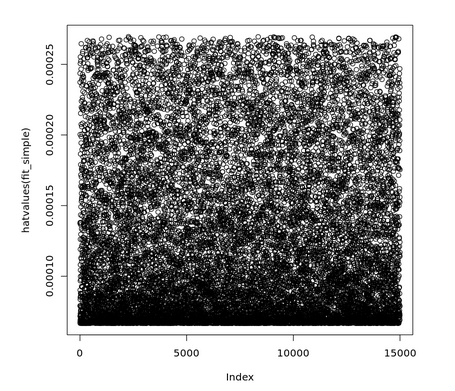
\includegraphics[width=1\linewidth]{lab2/obraz6.png}
    \caption{Podsumowanie LDA}
    \label{fig:enter-label}
\end{figure}

Prawdopodobieństwo przynależności do klasy wynosi około 14.4\%. Jeśli weźmiemy pod uwagę, że mamy 7 możliwych klas, to będziemy w stanie wywnioskować, że zbiór jest zbalansowany pod względem ich liczności.

Proporcja błędu to z kolei około 14.6\% - lepiej niż przy regresji logistycznej.

\subsection{Metoda QDA}
Przeprowadźmy analogiczną analizę przy pomocy \textbf{QDA}:

\begin{Rcode}
dir_qda <- list()
dir_qda$fit <- qda(Type_of_Renewable_Energy_1 ~ Energy_Production_MWh + Energy_Storage_Capacity_MWh, data = energy_data, subset = train)

print(dir_qda$fit)

dir_qda$predicted <- predict(dir_qda$fit, test)
predicted_classes <- dir_qda$predicted$class

actual_classes <- test$Type_of_Renewable_Energy_1
num_errors <- sum(predicted_classes != actual_classes)
total_samples <- length(actual_classes)

proportion_of_errors <- num_errors / total_samples
print(proportion_of_errors)
\end{Rcode}

\begin{figure}[H]
    \centering
    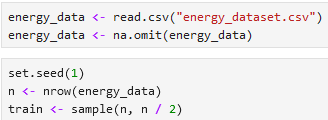
\includegraphics[width=1\linewidth]{lab2/obraz7.png}
    \caption{Podsumowanie QDA}
    \label{fig:enter-label}
\end{figure}

Proporcja błędów jest w tym przypadku taka sama, jak w LDA.

\subsection{Metoda kNN}
Na koniec sprawdźmy wyniki dla metody \textbf{kNN}, dla różnych wartości parametru \textbf{k}. W tym przypadku lekko modyfikujemy zbiory:

\begin{Rcode}
train_set <- energy_data[train, c("Energy_Storage_Capacity_MWh", "Energy_Production_MWh")]
test_set <- energy_data[!train, c("Energy_Storage_Capacity_MWh", "Energy_Production_MWh")]
renewable_energy_train <- energy_data$Type_of_Renewable_Energy_1[train]
Type_of_Renewable_Energy_1_test <- energy_data$Type_of_Renewable_Energy_1[!train]  
\end{Rcode}

Używamy kNN w pętli:
\begin{Rcode}
dir_knn <- knn(train_set, test_set, renewable_energy_train, k = k)
num_errors <- sum(dir_knn != Type_of_Renewable_Energy_1_test)
total_samples <- length(Type_of_Renewable_Energy_1_test)
\end{Rcode}

Zależność proporcji błędu od ilości parametrów:

\begin{figure}[H]
    \centering
    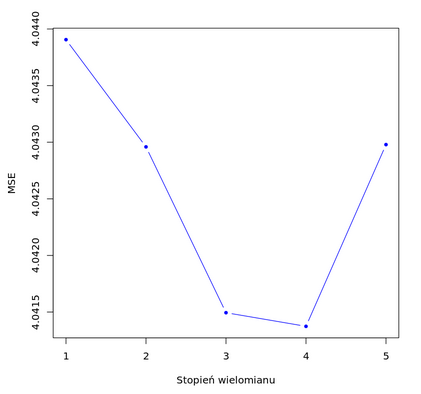
\includegraphics[width=1\linewidth]{lab2/obraz8.png}
    \caption{Wyniki dla kNN}
    \label{fig:enter-label}
\end{figure}

Dla \( k \geq 2 \) widzimy wartości wyższe lub zbliżone do regresji logistycznej. Dla wartości \( k \leq 8 \) wartości są najlepsze ze wszystkich metod.

